\documentclass{beamer}
\usepackage{graphicx}
\usepackage[outputdir=./target]{minted}
\usepackage[utf8]{inputenc}

\usetheme{Madrid}
\usecolortheme{dolphin}

\graphicspath{ {images/} }

\title{Degasolv}
\subtitle{A Generic Dependency Resolver}
\author{Daniel Jay Haskin}
\begin{document}
\begin{frame}
  \titlepage
\end{frame}
\begin{frame}
  \centerline{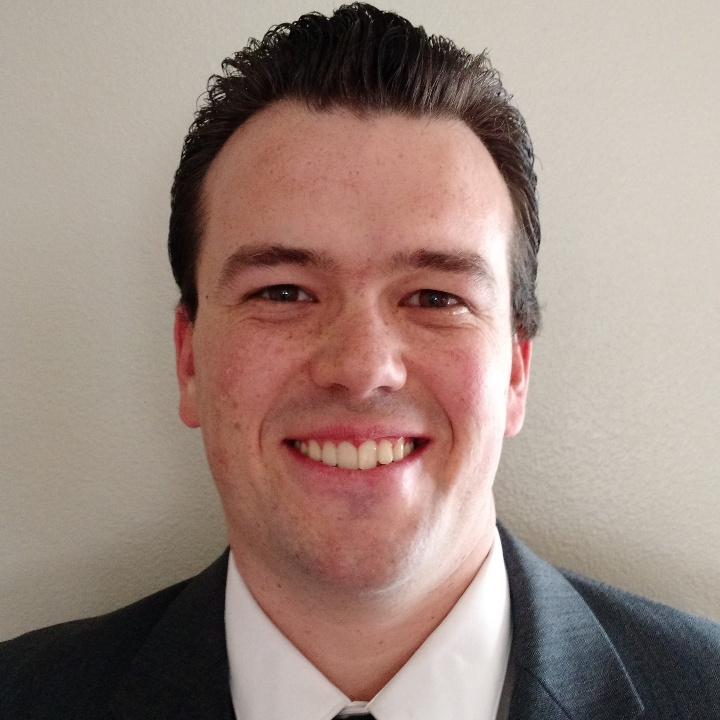
\includegraphics[scale=0.15]{DanielHaskin-small.jpg}}
  \center{
    Daniel Jay Haskin \\
    @djhaskin987
  }
\end{frame}
\begin{frame}[fragile]
  \frametitle{Dependencies Are The Worst}

\end{frame}
\begin{frame}
  \frametitle{Why Degasolv?}
  \begin{itemize}
  \item Some languages/technologies don't have a dependency manager
    \pause
  \item Cross-technology dependencies
    \pause
  \item Deal with site-specific quirks
  \end{itemize}
\end{frame}
\begin{frame}
  \frametitle{Overview}
  \begin{itemize}
  \item \texttt{generate-card}: Generate a ``card file'' which represents a package
  \item Upload the card file to a NAS or other central file share
  \item \texttt{generate-index}: Generate a ``repository index'' based on the card files in the central file share
  \item \texttt{query-repo}: Inspect what packages exist in the repository
  \item \texttt{resolve-locations}: Using repository indices, find the locations \\
    of packages and their dependencies
  \end{itemize}
\end{frame}

\begin{frame}
  \frametitle{What is a ``package''?'}
  \begin{itemize}
  \item A name
  \item A version
  \item A URL
  \item A list of dependencies
  \end{itemize}
\end{frame}
\begin{frame}
  \frametitle{\texttt{generate-card} Overview}
  \begin{itemize}
  \item Generates ``card'' files, which contain data about a particular package
  \item Keeps track of dependency information indepently of actual package file contents
  \item Degasolv ``stays out of your way''
  \end{itemize}
\end{frame}
\begin{frame}[fragile]
  \frametitle{\texttt{generate-card} Example}
  \begin{minted}{bash}
    java -jar \
        ./degasolv-1.0.3-SNAPSHOT-standalone.jar \
        generate-card \
        -i "e" \
        -v "1.8.0" \
        -l "https://example.com/repo/e-1.8.0.zip" \
        -C $PWD/e-1.8.0.zip.dscard
  \end{minted}
\end{frame}
\begin{frame}[fragile]
  \frametitle{\texttt{generate-card} Output: The \texttt{*.dscard} File}
  \begin{minted}{clojure}
    ; Filename: e-1.8.0.dscard
    #degasolv.resolver/PackageInfo
    {
      :id "e",
      :version "1.8.0",
      :location "https://example.com/repo/e-1.8.0.zip",
      :requirements []
    }
  \end{minted}
\end{frame}
\begin{frame}
  \centerline{\color{blue}\Large \texttt{generate-card} Demo}
\end{frame}
\begin{frame}
  \frametitle{\texttt{generate-index} Overview}
\end{frame}
\begin{frame}
  \frametitle{\texttt{generate-index} Example}
\end{frame}
\begin{frame}
  \centerline{\color{blue}\Large \texttt{generate-index} Demo}
\end{frame}
\begin{frame}
  \frametitle{\texttt{query-repo} Overview}
\end{frame}
\begin{frame}
  \frametitle{\texttt{query-repo} Example}
\end{frame}
\begin{frame}
  \centerline{\color{blue}\Large \texttt{query-repo} Demo}
\end{frame}
\begin{frame}
  \frametitle{\texttt{resolve-locations} Overview}
\end{frame}
\begin{frame}
  \frametitle{\texttt{resolve-locations} Example}
\end{frame}
\begin{frame}
  \centerline{\color{blue}\Large \texttt{resolve-locations} Demo}
\end{frame}
\begin{frame}
  \centerline{\color{blue}\Large Multi Technology Demo}
\end{frame}
\begin{frame}
  \centerline{\color{blue}\Large Native Code Demo}
\end{frame}
\begin{frame}
  \frametitle{Summary}
\end{frame}
\begin{frame}
  \frametitle{Community}
\end{frame}
\begin{frame}
  \frametitle{Future Directions}
  \begin{itemize}
  \item Resolution directly from different types of repositories
  \item Homebrew: https://github.com/Homebrew/brew/blob/master/docs/Formula-Cookbook.md
  \item RPM, Debian packages, bintray
  \item Artifactory plugin
  \end{itemize}
\end{frame}
\begin{frame}
  \frametitle{Further Reading}
  \begin{itemize}
  \item Kill Your Dependencies http://www.mikeperham.com/2016/02/09/kill-your-dependencies/
  \item Embracing Conway's Law https://wingolog.org/archives/2015/11/09/embracing-conways-law
  \end{itemize}
\end{frame}
\begin{frame}
  \centerline{\color{blue}\Large Questions}
\end{frame}
\end{document}
